\documentclass[9pt,shortpaper,twoside,web]{ieeecolor}
\usepackage{generic}
\usepackage{cite}
\usepackage{amsmath,amssymb,amsfonts}
\usepackage{algorithmic}
\usepackage{graphicx}
\usepackage{textcomp}

\def\BibTeX{{\rm B\kern-.05em{\sc i\kern-.025em b}\kern-.08em
    T\kern-.1667em\lower.7ex\hbox{E}\kern-.125emX}}
\markboth{\journalname, Research and documentation project}
{Author \MakeLowercase{\textit{et al.}}: A brief introduction in object localization algorithms for the researching project  (February 2018)}

\begin{document}
\title{
A brief introduction in object recognition algorithms \\
for researching project  \\ 
(February 2018)}
\author{Iordache-Stoicescu Laurențiu \\ and \\ Dumitru George}

\maketitle


\begin{abstract}
Object recognition plays a very important role in computer vision based applications. This type of application 
are vital for autonomous systems and for industrial applications. In this paper are presented some popular approaches 
of object recognition such as PCA, SIFT, SURF, FAST etc. Furthermore, the pros and cons of object recognition algorithms 
are described and a classification of those algorithms by the processing based method was attempted. Finally, these 
algorithms are compared in terms of accuracy and robustness.
\end{abstract}

\begin{IEEEkeywords}
ANN - Artificial Neural Network
BRIEF – Binary Robust Independent Elementary Features; 
BRISK – Binary Robust Invariant Scalable Keypoints; 
DoG – Difference Of Gaussian; 
FAST – Features from Accelerated Segment Test; 
FREAK – Fast Retina Keypoint;
FLANN - Fast Library for Approximate Nearest Neighbors;
HoG - Histogram of Gaussian
LOG – Laplacian Of Gaussian; 
ORB – Oriented fast and Rotated BRIEF; 
PCA - Principal Component Analysis;
RGB – Red Green Blue; 
SIFT – Scale-Invariant Feature Transform; 
SURF – Speed Up Robust Features; 
\end{IEEEkeywords}

\section{Introduction}
\label{sec:introduction}

Over the last decades, image feature detectors and descriptors have become popular tools in the computer vision community and they are being applied widely in a large number of applications. Image representation, image classification and retrieval, object recognition and matching, 3D scene reconstruction motion tracking, texture classification, biometrics systems etc. 

In order to establish correspondences among a collection of images, it is necessary to find a set of points in each image that can describe the image.
In object recognition tasks, interest points described from the query image are matched with the descriptions of interest points from the train images set. The train image giving maximum correspondence is considered to be the best representation of the query image.

Images can be analyzed in two ways. First method implies extracting global features from image content representation and the second and the more precise one implies local feature extraction. Global features aim to describe an image using all the pixels values for example color or texture, while local features aim to detect the interest points of the image and describe them in such a manner that they can be matched in other representations of the same scene. In order to recognize distinct objects we can train artificial neural networks in order to find specific patterns in the interest points.

\subsection{Appearance-Based Method}
Appearance-based object recognition strategy is popular for face and handwriting recognition. For this strategy is needed a set of training reference images with a highly correlation between them. For example a data set containing lots of images of faces which are highly correlated and subsets of random images which are not correlated at all with the face images data set. This data set is compressed using dimension reduction techniques in order to obtain a lower dimension subspace, also called eigenspace. Parts of the new input images are projected on the eigenspace and then correspondence is examined \cite{b1}.

\subsection{Feature-Based Method}
Over the last decades, image features and descriptors have become very powerful tools in computer vision applications. Those are used in a large number of applications such as: Object recognition and matching, image classification, 3D scenes reconstruction, motion tracking, biometric systems etc.

The first step of a feature-based object recognition system is to detect interest locations int the sample image and describe them. Once the interest locations are described, they can be matched with the descriptions from the test image in order to identify the same interest locations. Every input image is searched for a specific type of feature, this feature is then compared to a database containing models of the objects in order to verify if there are recognised objects. Usually, the interest points are represented by lines, corners or bloobs. Those are the points that can describe an object in the easiest way.

\subsection{Pattern Matching Method}
Pattern matching methods are often used because they are simple to implement. This technique consists in finding small patches of an image that match a template image.

The computation formula is described in Eq(1). The squared differences between an image patch I and a template M are summed pixelwise. A threshold has to be provided in order to let the algorithm decide whether a template matched and an object was recognised \cite{b1}. 

\begin{equation} 
\label{eq1}
r(x,y) = \sum\limits_{i}^M \sum\limits_{j}^M (I (x + i, y + i) - M(i, j))^2
\end{equation}

In order to enhance the distortion and light changes effects, the result can be adjusted like in the Eq(2). where n is the number of pixels in the template.

\begin{equation}
\label{eq2}
\frac{ \sum IM - \sum I * \sum M}
{ \sqrt{(n \sum I^2 - ( \sum I)^2) (n \sum M^2 - ( \sum M)^2)}}
\end{equation}

The template matching method is used in application such as traffic sign recognition. As this approach has lots of disadvantages such as problems with
occlusion, rotation, scaling, different illuminations and so on, it will not be given further attention in this work \cite{b1}.

\subsection{Artificial Neural Networks}
Artificial neural networks are computing systems inspired by the biological neural networks that constitute animal brains. Those systems learn tasks by considering examples without specific programming. Such models consists of several layers in which each layer is composed of a certain number of neurons. The input and output layers are the mandatory layers of a neural network. Normally hidden layers are included in order to be able to learn more complex tasks such as object recognition.

\begin{figure}[htb]
\centerline{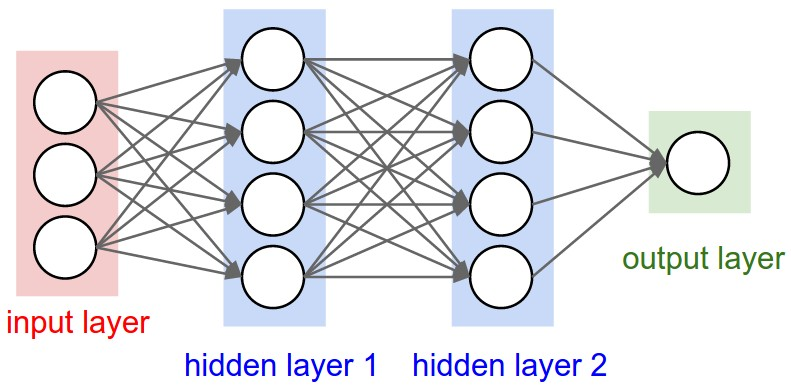
\includegraphics[width=\columnwidth]{res/fig/ann.jpg}}
\caption{Neural network with one input layer, two hidden layers and one output layer.}
\label{fig1}
\end{figure}

In image recognition, they might learn to identify images that contain certain objects by analyzing a big set of images of that certain object and

\section{Feature-Based Method}

In order to establish correspondences among a collection of images is needed to identify a set of salient points in each each image. In a classification task, the descriptions of each detected keypoint of the object's image is matched with all the train images descriptions of keypoints. The trained image which giving maximum correspondence is considered the best match. The matching can be given by measuring the euclidean distance.

The basic idea is to first detect interest regions (keypoints) that are covariant to a class of transformations \cite{b2}. Then, for each detected regions, an invariant feature vector representation (i.e., descriptor) is built. For each keypoint will be computed a descriptor vector that will describe the patch surrounding the point. With those pairs of keypoints and descriptors we can find the points that match a specific descriptor in other image.

\subsection{Feature Detectors}

A local feature is defined as an image pattern which differs from its immediate neighborhood. The goal of feature detectors and extractors is to obtain and encode a set of local measurements that capture the essence of the object that we want to describe. The following properties are important for utilizing a feature detector in computer vision applications:

\begin{itemize}

\item Robustness, the feature detection algorithm should be able to detect the same feature locations independent of scaling, rotation, shifting, photometric deformations, compression artifacts, and noise.

\item Repeatability, the feature detection algorithm should be able to detect the same features of the same scene or object repeatedly under variety of viewing conditions.

\item Accuracy, the feature detection algorithm should accurately localize the image features (same pixel locations), especially for image matching tasks, where precise correspondences are needed to estimate the epipolar geometry.

\item Generality, the feature detection algorithm should be able to detect features that can be used in different applications.

\item Efficiency, the feature detection algorithm should be able to detect features in new images quickly to support real-time applications.

\item Quantity, the feature detection algorithm should be able to detect all or most of the features in the image. Where, the density of detected features should reflect the information content of the image for providing a compact image representation. \cite{b2}

\end{itemize}

Feature detectors are broadly classified into three categories: single-scale detectors, multi-scale detectors, and affine invariant detectors.

Single-scale detectors are defined by the following properties: Invatiant to image transformations such as rotation, translation, changes in illuminations and addition of noise. The main issue of this type of feature detector is incapability to handle scale changes therefore we must use multi-scale detectors in order to solve the scaling problem. Mulsti-scale detectors are as well invariant to image transformations and affine invariant. Further will be presented some popular feature detectors.
\\

\subsubsection{Harris Feature Detector}
Harris detector is a combined corner and edge detection operator that is commonly used to infer features and of an image and is a single-scale detector. It was first introduced in 1988 as an improvement of Moravec's corner detector. Compared to the previous one, Harris corner detector is more accurate in distinguishing between corners and edges.

By obtaining the variation of the autocorrelation (intensity variation) over all different orientations will converge to a more reliable detector in terms of detection and repeatability rate. The detector uses a $2 x 2$ symmetric auto-correlation matrix for features detecting.

\begin{equation}
\label{eq3}
M(x, y) = \sum\limits_{u, v} w(u, v) 
\begin{bmatrix}
I_x^2(x, y) & I_x I_y (x, y) \\
I_xI_y(x,y) & I_y^2(x, y) \\
\end{bmatrix}
\end{equation}

Where $I_x$ and $I_y$ are local image derivatives in the $x$ and $y$ directions, and $w(u, v)$ is a weighting kernel over the area $(u, v)$. In order to detect features, the eigenvalues of the matrix M are computed for each pixel. When the eigenvalues are large a corner is detected at the respective location. In case that just one eigenvalue is large a edge is detected. The representation of eigenvalues dimensions and feature detection is better represented in Figure 1

\begin{figure}[htb]
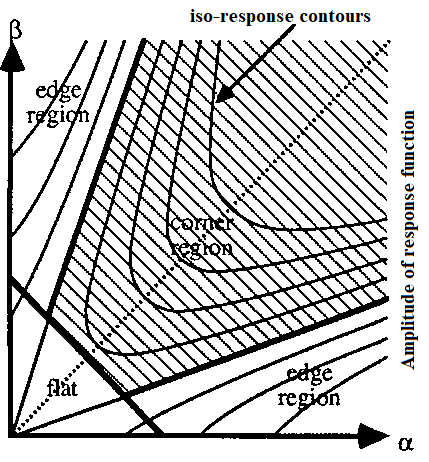
\includegraphics[width=0.9\columnwidth]{res/fig/Harris.png}
\caption{Classification of image points based on the eigenvalues of the autocorrelation matrix $M$ \cite{b3}}
\label{fig2}
\end{figure}

In order to find features, the eigenvalues are computed for each pixel. Constructing the response map can be done by calculating the cornernes measure $C(x, y)$ for each pixel $(x,y)$ using the

\begin{equation}
\label{eq4}
C(x, y) = det(M) - K(trace(M))^2
\end{equation}

where 


\begin{equation}
\label{eq5}
det(M) = \lambda_1 * \lambda_2, and trace(M) = \lambda_1 + \lambda_2
\end{equation}

The K is an adjusting parameter and $\lambda_1, \lambda_2$ are the eigenvalues of the auto-correlation matrix. The process of computing the eigenvalues is computational expensive because of the square root. Harris suggested using this cornerness measure that combines the two eigenvalues in a single measure. The non-maximum suppression should be done to find local maxima and all non-zero points remaining in the cornerness map are the searched corners.
\\

\subsubsection{FAST Feature Detector}

Features for accelerated segment test(FAST) is a  single-scale corner detection method which is used to extract feature points. The FAST corner detector was originally developed by Edward Rosten and Tom Drummond and was published in 2006. The biggest advantage of FAST is, as the abbreviation of it's name says it, that is a fast processing tool.

The process of corner detection consist by applying a segment test to each pixel by considering a sampling circle of 16 pixels around the corner candidate pixel as a base of computation. If a set of $n$ neighboring pixels in the Bresenham circle with the radius $r$ are all brighter or darker than the candidate pixel plus a threshold value $t$, then the considered pixel is classified as a corner as exemplified in figure 3.

\begin{figure}[htb]
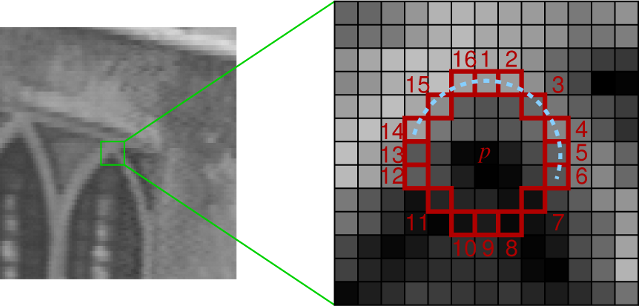
\includegraphics[width=\columnwidth]{res/fig/FAST.png}
\caption{Corner detection using Bremenham sampling circle applied to a corner candidate.}
\label{fig3}
\end{figure}

A high-speed test to exclude all non-corners points is used. In this test only pixels 1, 5, 9 and 13 are examined. A corner can exist only if three of those pixels are brighter or darker than the considered pixel $p$. Based on this statement, the computation time is enhanced by fast eliminating the pixels that are not corners. Although the high speed test yields high performance, it has several weakness. An improvement for these limitations and weakness is achieved using a machine learning approach. The ordering of questions used to classify a pixel is learned by using the ``well-known decision tree algorithm (ID3)'', which speeds this step up significantly \cite{b2}.
\\

\subsubsection{Laplacian of Gaussian}

Laplacian of Gaussian (LoG) is a common blob detector. The Laplacian is a 2D isotropic measure of the second spatial derivative of an image used to find areas of rapid change in images (edges). Since derivative filters are very sensitive to noise, it is common to smooth the image using a Gaussian filter before applying the Laplacian. This two-step process is called the Laplacian of Gaussian operation.

Given an input image $I(x, y)$, the scale space representation of the image is defined by $R(x, y, \sigma)$ is obtained by convolving the image with a variable Gaussian kernel $G(x, y, \sigma)$ where

\begin{equation}
\label{eq6}
R(x, y, \sigma) = G(x, y, \sigma) * I(x, y)
\end{equation}

and

\begin{equation}
\label{eq7}
G(x, y, \sigma) = \frac{1}{2 \pi \sigma^2} e^{\frac{-(x^2 + y^2)}{2\sigma^2}}
\end{equation}

To include a smoothing Gaussian filter, combine the laplacian and the Gaussian functions to obtain a single equation/ The LoG operator takes the second derivative of the image. The LoG will give zero where the image is uniform and where changes occurs, the Log will give a positive response on the darker side and a negative response on the lighter side.

\begin{equation}
\label{8}
LoG(x, y) = \nabla^2G(x, y, \sigma) - \frac{1}{\pi \sigma^4}( 1- \frac{x^2 + y^2}{2 \sigma^2}) e^{- \frac{x^2 + y^2}{2 \sigma^2}}
\end{equation}

 However, the operator response is strongly dependent on the relationship between the size of the blob structure and the size of the smoothing Gaussian kernel \cite{b2}. The scale control is achieved by changing the standard deviation $\sigma$. The computation of LoG operators is time consuming so, as an alternative to this method is used Difference of Gaussian (DoG).
\\

\subsubsection{Difference of Gaussian}
Difference of Gaussians (DoG) represents a feature enhancement algorithm that involves the subtraction of one blurred version of an original image from another one less blurred. The blurred images are created as in the Laplacian of Gaussian algorithm by convolving the original image with a variable Gaussian kernel.

Blurring an image with a Gaussian kernel suppresses only high-frequency spatial information. Subtracting one image from another preserves spatial information that lies between the range of frequencie that are preserved in the two blurred images. Thus, the DoG is a band-pass filter that discards all but a handful of spatial frequencies that are present in the original image. This approach is used in scale-invariant transform (SIFT) algorithm. In this context, the DoG gives a close approximation to the Laplacian of Gaussian and is more computational friendly because it can be computed without convolution.

\subsection{Feature Descriptors}
After detecting a interest point from an image at a certain location $p(x, y)$, the neighborhood of p needs to be described in a suitable manner in order to be discriminative and insensitive to local image deformations. In general, the problem we are focusing on is that of comparing two image patches and measuring their similarity. There are a large number of image feature descriptors in the literature. Further will be presented some frequently used descriptors.
\\

\subsubsection{Scale Invariant Feature Transform}
Scale Invariant Feature Transform (SIFT) is an algorithm used to describe keypoints detected with int the image using the DoG operator. For each interest point, a feature vector is extracted. The algorithm computes the orientation of the image over a number of scales and over a patch around the interest point in order to provide rotation invariance.

The SIFT descriptor builds a histogram of gradient magnitudes and orientations for a 16 x 16 pixels region around each interest point using its scale to select the level of Gaussian blur for the image. After, a set of orientation histograms with samples from a 4 x 4 subregion of the original $16 x 16$ patch is created. Each one have eight orientations bins \cite{b4}.

\begin{figure}[htb]
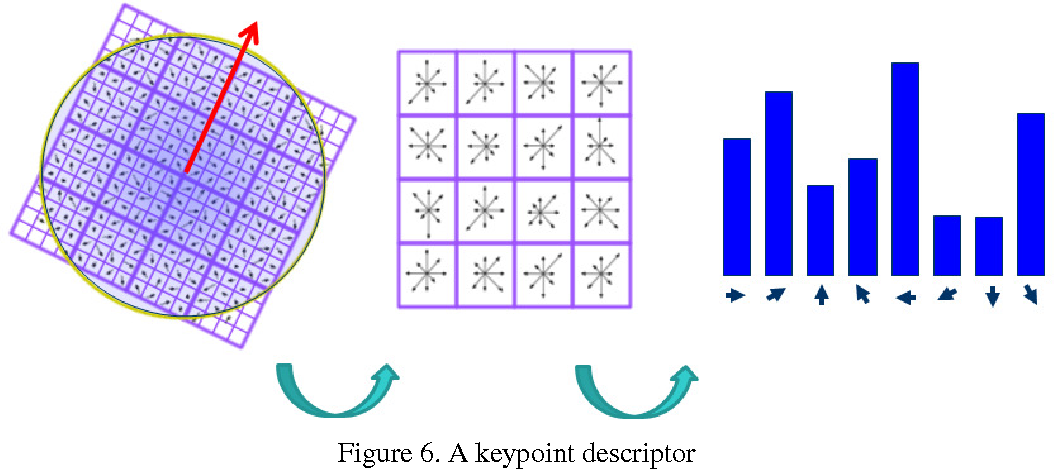
\includegraphics[width=\columnwidth]{res/fig/SIFT.png}
\caption{Representation of SIFT descriptor for a 16 x 16 pixel patch weighted by a Gaussian falloff indicated by overlaid circle.}
\label{fig4}
\end{figure}

The magnitude of each point is wighted with a Gaussian weighting function in order to give  and less weight to gradients far from the interest point. There fore, feature vector dimension is 128 (4 x 4 x 8). Finally, the feature vector is normalized to unit length. The normalization offers invariance to affine changes and illumination. Some changes can occur due to camera saturation or similar effects. A good way to combat these effects is to threshold the values in the feature vector to a maxim value of 0.2 \cite{b3}.

The standard  SIFT descriptor has the following advantages: it avoid problems du to boundary effects-smooth changes in location thanks to the representation of characteristics, is fairly compact thanks to the 128 elements vector, orientation and scale don't cause big changes in the descriptor vector. These characteristics are evidenced in excellent matching performance under different scales, rotations and lighting. It's main disadvantage is the processing speed due to high dimensionality.
\\

\subsubsection{Speed-Up Robust Features Descriptor}
Speed-Up Robust Features Descriptor (SURF) is an alternative to SIFT. This algorithm presents a better computational speed and a better robustness while keeping the advantages of SIFT.


The feature detection is based on simple 2D filters, it uses a scale invariant blob detector based on the determinant of Hessian matrix for both scale selection and location \cite{b2}. 
\begin{figure}[htb]
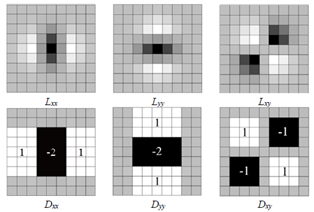
\includegraphics[width=\columnwidth]{res/fig/SURF.png}
\caption{Representation of SIFT descriptor for a $16 x 16$ pixel patch weighted by a Gaussian falloff indicated by overlaid circle.}
\label{fig5}
\end{figure}
While SIFT uses approximated LoG for finding scale-spaces, SURF approximates LoG with Box Filter. One big advantage of this approach is that, convolving with box filters can be done with the help of integral images and it can be done in parallel for different scales.

The SURF descriptor begins by constructing a square region centered on the detected interest point ant orientated along its main orientation. Th size of the window is $20s$ with $s$ equals to the scale at which the feature is detected. After considering a window, is divided into smaller 4 x 4 sub-windows and for each one Haar wavelet response in the vertical and horizontal directions are computed at a 5 x 5 sampled points as shown in Figure 6.

\begin{figure}[htb]
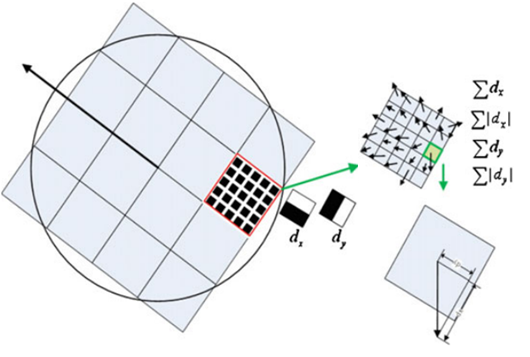
\includegraphics[width=\columnwidth]{res/fig/SURFsampling.png}
\caption{Haar wavelet response sampling weighted by a Gaussian falloff indicated by overlaid circle and orientation computing.}
\label{fig6}
\end{figure}

The wavelet responses are weighted with a Gaussian window centered on the interest point in order to increase the robustness against geometric deformations and errors generated by localization. The responses $d_x$ and $d_y$ are summed up for each sub-window and inserted in a feature vector $v$ where

\begin{equation}
\label{eq9}
v = ( \sum d_x , \sum |d_x|, \sum d_y, \sum |d_y| ) 
\end{equation}

The feature vector is computed for each sub-window, resulting a feature descriptor of length 4 x 4 x 4 = 64 dimensions. The feature descriptor is further normalized to a unit vector in order to reduce illumination effects \cite{b5}.

The main advantage of SURF descriptor compared to SIFT is the processing speed. This is given by the feature vector's dimension, it uses only 64 values in order to describe an interest point.

Beside the disadvantage of computational complexity of both SURF and SIFT descriptors they have another one that may affect the decision to choose one of them, they are patented by the institutions so in order to use them you must pay.
\\

\subsubsection{Binary descriptors}
Considering the fact that SIFT and SURF descriptors are based on HoG which implies computing gradients for every pixel from the patch surrounding the interest point, they are costly from the perspective of time and processing resources. This is where binary descriptors come in handy. 

The principle on which they are based is to encode most of the information of a patch just by comparing intensity images. This can be done very fast only using the Hamming distance as a distance measure between two binary vectors and then matching between two patch descriptions. The matching process can be done very easy just by computing the sum of the XOR operation between two binary strings.

In general, binary descriptors have three constituent parts: A sampling pattern, orientation compensation algorithm and a sampling pairs pattern. In order to describe a patch is needed a sampling pattern of a window of various size centered on the interest point.

\begin{figure}[htb]
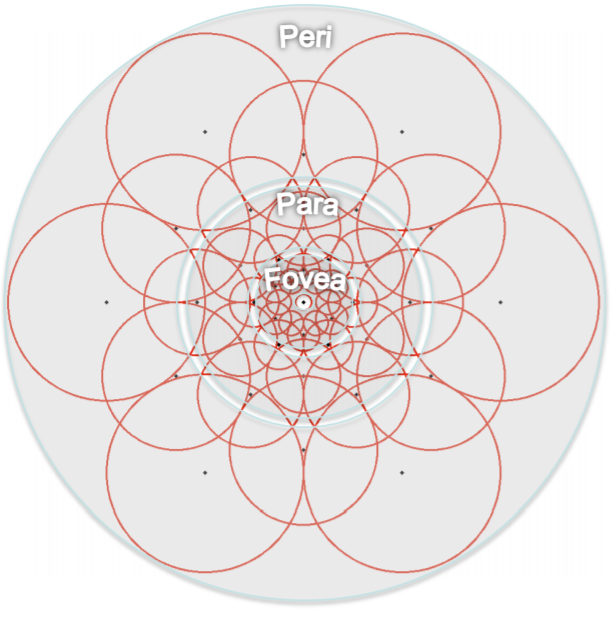
\includegraphics[width=0.5\columnwidth]{res/fig/FREAKsampling.png}
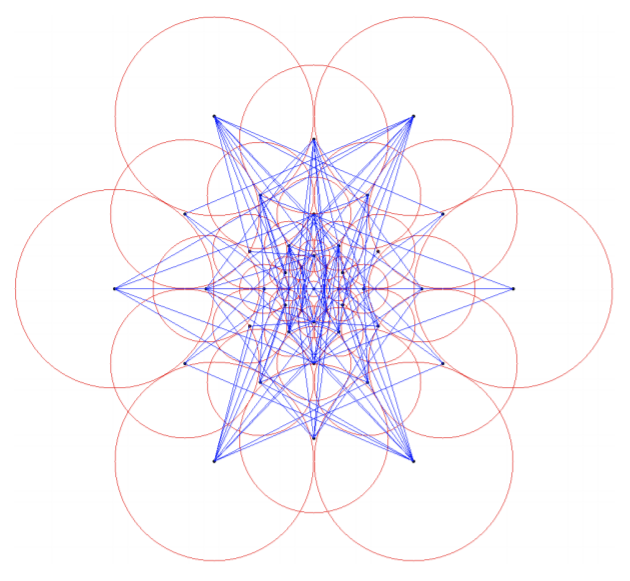
\includegraphics[width=0.5\columnwidth]{res/fig/FREAKsaplePairs.png}
\caption{FREAK sampling pattern and sample pairs generating algorithm \cite{b7}.}
\label{fig7}
\end{figure}

With the resulted samples from the patch the algorithms consider a number of pairs of points. For each pair the intensity value is compared. If the first value is bigger it will be represented as '1' in the description vector else will be represented as a '0'. In order to compare two patches it is enough just to count the number of bits where description vector differs. This is done applying

\begin{equation}
\label{eq10}
v = \sum (d_x \oplus d_y) 
\end{equation}

where $d_x$ is the description vector of the known interest point $d_y$ is the description vector of the supposed point in another image. Each binary descriptor has its own sampling patterns, pairs creating patterns and orientation deduction algorithms. Further will be briefly presented some binary algorithms particularities.\\


\paragraph{BRIEF}
BRIEF was the first binary descriptor published. It doesn't have any orientation algorithm or elaborated sampling pattern. BRIEF take only the information from single pixels in order to build the descriptor so in order to be less sensitive to noise the image must be smoothed first.

In order to build the descriptor it must define a sampling pattern in order to determine $n$ pairs $(x_i,y_i)$. The authors consider five methods to determine these vectors \cite{b8} :

\begin{itemize}
\item $X$ and $Y$ are uniform distributed over the patch.

\item Locations are Gaussian sampled, this means that the center region has more samples that the marginal areas.

\item $X$ and $Y$ are sampled using two distinctive Gaussian sampling patterns that vary in standard deviations. This forces the samples to be more local.

\item $X$ and $Y$ are randomly sampled from discrete location of a coarse polar gird.

\item For each pair, the $X$ member will be the interest point and $Y$ takes all possible values on a coarse polar grid centered on the interest point.
\end{itemize}

As with all binary descriptors, computing the description vector consists in comparing the two pairs of samples. The process of matching two interest point is the same, just using the XOR operation between the two description vectors.
\\

\paragraph{ORB}
ORB descriptor is a bit similar to BRIEF, it doesn't have an elaborate sampling pattern ass BRISK or FREAK. However, there are two main differences between ORB and BRIEF:

\begin{itemize}
\item ORB make use of a orientation compensation mechanism, this confers it rotation invariant.

\item ORB auto-adapts the sampling pairs in order to obtain the optimal one.
\end{itemize}

ORB is basically a fusion of FAST keypoint detector and BRIEF descriptor with many modifications to enhance the performance. First it use FAST to find keypoints, then apply Harris corner measure to find top N points among them. It also use pyramid to produce multiscale-features. But one problem is that, FAST doesn’t compute the orientation  \cite{b9}.

It computes the intensity weighted centroid of the patch with located corner at center. The direction of the vector from this corner point to centroid gives the orientation. To improve the rotation invariance, moments are computed with x and y which should be in a circular region of radius r, where r is the size of the patch \cite{b9}.
\\

\paragraph{BRISK}
The BRISK descriptor is different from BRIEF and ORB by having a defined sampling pattern. This consists in concentric sampling circles. For each sampling circle we apply Gaussian smoothing in order to reduce the noise sensibility. The standard deviation of each circle vary in depending on how close is from the center.

\begin{figure}[htb]
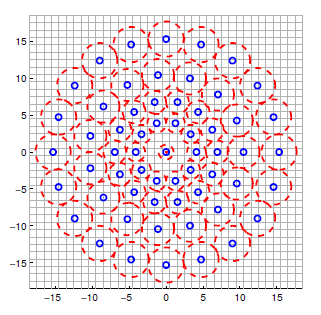
\includegraphics[width=0.5\columnwidth]{res/fig/BRISKsampling.png}
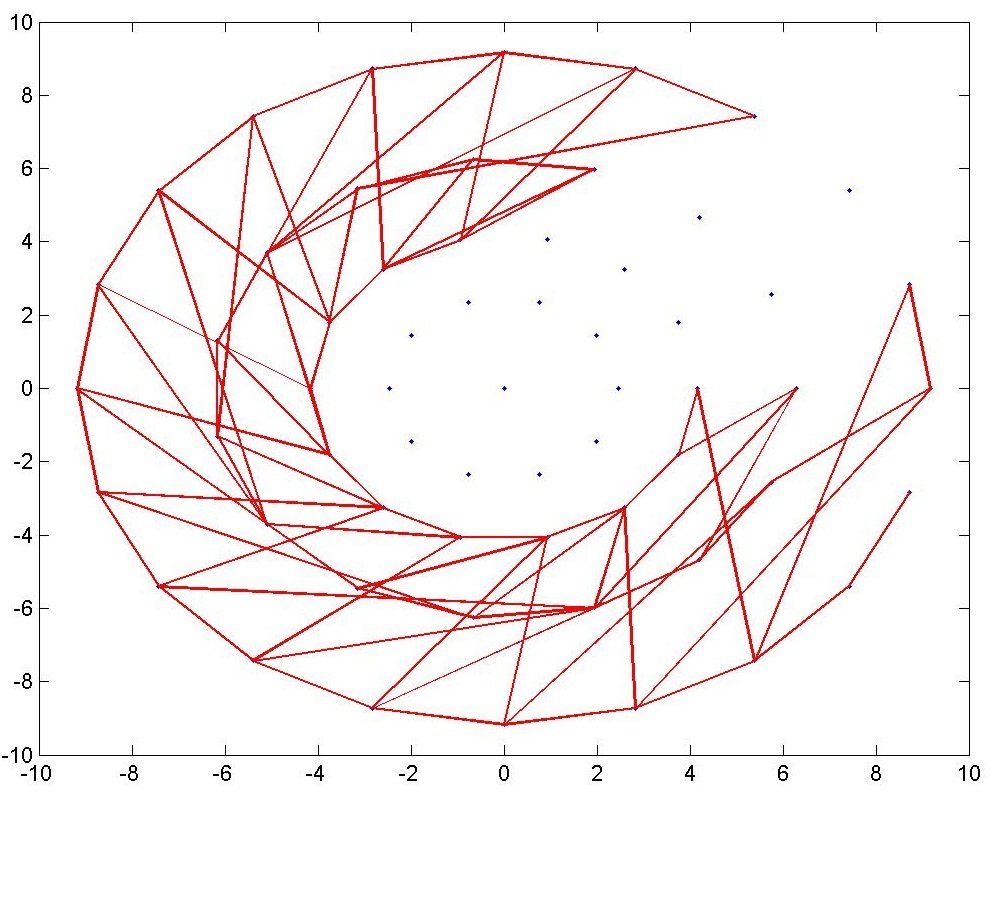
\includegraphics[width=0.5\columnwidth]{res/fig/BRISKsamplePairs.jpg}
\caption{BRISK sampling pattern and sample pairs generating algorithm \cite{b6}.}
\label{fig8}
\end{figure}

When creating the pairs of samples we distinguish short distance pairs and long distance pairs. Short pairs are pairs of sampling that are used for the intensity comparisons that build the descriptor and long pairs are used to compute the orientation of the patch.
\\

\paragraph{FREAK}
FREAK is a descriptor with a handcrafted sampling pattern that uses machine learning techniques to learn the optimal set of sampling pairs \cite{b6}.

Many sampling patterns are possible to compare pixel intensities. As we have seen, BRIEF uses random pairs, ORB uses learned pairs and BRISK uses a circular pattern where points are equally spaced on circles concentric.FREAK suggests to use the retinal sampling grid which is also circular with the difference of having higher density of points near the center. The density of points drops exponentially to the extremities as can be seen in Figure 7. Each sample point is smoothed with a Gaussian with the standard deviation given by the radius of the corresponding circle.

A possible strategy of choosing sampling points is to follow the ORB approach and try to learn the pairs by maximizing variance of the pairs and taking pairs that are not correlated in order to maximize the sampled information. One of the many sampling patterns possible is illustrated in figure 7.

FREAKS takes advantage of this coarse-to-fine structure to speed up the matching using a cascade approach. When matching two descriptors, we first compare only the first 128 bits. If the distance is smaller than a selected threshold, we further continue the comparison until the next 128 bits. As a result, a cascade of comparisons is performed accelerating even further the matching as more than $90\%$ of the candidates are discarded with the first 128 bits of the descriptor \cite{b6}.

In order to compensate rotation changes, FREAK measures the orientation of the interest point by using a predefined set of 45 long distance symmetric sampling pairs similarly to BRISK descriptor.
\\

\begin{table}[htb]
\caption{Comparison of the Four Binary Descriptors}
\label{table1}
\setlength{\tabcolsep}{3pt}
\begin{tabular}{|p{0.10\columnwidth}|p{0.25\columnwidth}|p{0.35\columnwidth}|p{0.22\columnwidth}|}
\hline

Name&
Sampling pattern&
Orientation calculation&
Sampling pairs\\
\hline

BRIEF&
None&
None&
Random\\
\hline

ORB&
None&
Moments&
Learned pairs\\
\hline

BRISK&
Concentric circles with more points on outer rings&
Comparing gradients of long pairs&
Using only short pairs\\
\hline

FREAK&
Overlapping Concentric circles with more points on inner rings&
Comparing gradients of preselected 45 pairs&
Learned pairs\\
\hline

\end{tabular}
\label{tab1}
\end{table}

\subsection{Features Matching}
Features matching or generally image matching is the task of establishing correspondences between two images of the same scene. The matching is achieved by using the detected feature position (keypoint) and its descriptor.

A common approach to image matching consist in detecting a set of interest points, each associated with image descriptors of the image data. Once the features and descriptors are computed from two or more images the next step consist in establishing some preliminary feature matches between these images as shown in Figure 9.

\begin{figure}[htb]
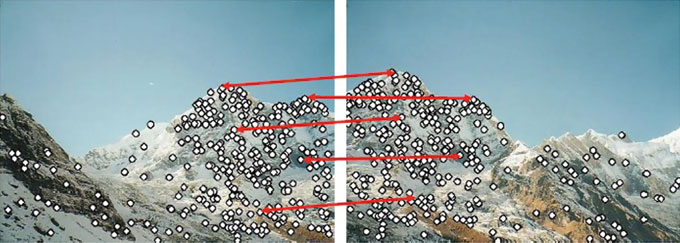
\includegraphics[width=\columnwidth]{res/fig/Matching.png}
\caption{Matching image regions based on their local feature descriptors \cite{b6}.}
\label{fig9}
\end{figure}

The problem of image matching can be solved as follows. Suppose that p is detected feature point with a feature detector associated with a descriptor
\begin{equation}
\label{eq11}
\Phi (p) = \{\phi_k(P) \quad | \quad  k = 1, 2, ..., K \} 
\end{equation}
where, for all K, the feature vector provided by provided by the $k$-th descriptor is
\begin{equation}
\label{eq12}
\phi_k(p) = (f_{1p}^l, f_{2p}^k, ..., f_{n_kp}^k)
\end{equation}

The task is to find the best correspondence $q$ in the other images from the set of $N$ interest points $Q = \{q_1, q_2, ..., q_N\} $ by comparing the description vector $\phi_k(p)$ with those of the points in the set $Q$.A distance measure between the two interest points descriptors $\phi_k(p)$ and $\phi_k(q)$ can be defined as
\begin{equation}
\label{eq13}
d_k(p,q) = |\phi_k(p) - \phi_k(q)|
\end{equation}

Based on the distance $d_k$, the interest points form the other images $Q$ are sorted in ascending order independently for each descriptor. A match between the pair of interest point $(p,q)$ is considered only if $p$ is the best match for q in relation to all the other points in the first image and $q$ is the best match for p in relation to all the other points in the second image \cite{b2}. To match vector based features we can use the nearest-neighbor matching in the feature space of the image descriptors in Euclidean norm. In order to reduce the ambiguity of the of matching candidates correspondence, the ratio between the distances of the nearest and the next nearest image descriptor must be less than a given threshold. Two algorithms have been found to be the most efficient: the randomized k-d forest and the fast library for approximate nearest neighbors (FLANN) \cite{b2}.

On the other hand, these algorithms are not suitable for binary descriptors. Binary features are matched using Hamming distance computed with a bitwise XOR operation followed by a bit count on the result after determining the orientation of the patch and rotating it to match the orientation of the searched one.

The performance of matching methods based on interest points and descriptors depends on both the properties of the interest point and the choice of feature descriptor. The detectors and descriptors should be selected based on the image contents and application types. For instance, for a application that shall detect and track blobs it must use a blob detector not a corner detector and vice versa.

\section{Artificial Neural Networks}
An Artificial Neural Network (ANN) is an information processing model that is inspired by the way  biological nervous systems process information, such as the brain. It is composed of a large number of highly interconnected processing elements (neurons) working in unison to solve specific problems. 

Neural networks can be used to extract patterns and detect trends that are too complicated to be noticed by either humans or other computer techniques. A trained neural network can be thought of as an "expert" in the category of information it has been given to analyze because we feed him with a lot of information from the areas of interest.

Other advantages include:

\begin{itemize}

\item Adaptive learning: ability to learn how to do tasks based on the data  given for training or initial experience;

\item Self-Organizing: the capability of organizing or representing the information it receives during learning time in a useful manner;

\item Real Time Operation: computations may be carried out in parallel, and special hardware devices are being designed and manufactured which take advantage of this capability;

\item Fault Tolerance via Redundant Information Coding: Partial destruction of a network leads to the corresponding degradation of performance. However, some network capabilities may be retained even with major network damage.

\end{itemize}

\subsection{Human Object recognition}
Much of the power of artificial intelligence stems from cloning the human behavior. One attempt to understand human object recognition ist the theory of $Recognition By Components$. The basis for this theory is that human primary way of classifying objects is by identifying their components and the relational properties among these components, rather than by features as texture or color. Recognition is based on decomposition of an object in geons and utilizes the relation among entities, in the form of orientation, distance, size and connections.

\begin{figure}[htb]
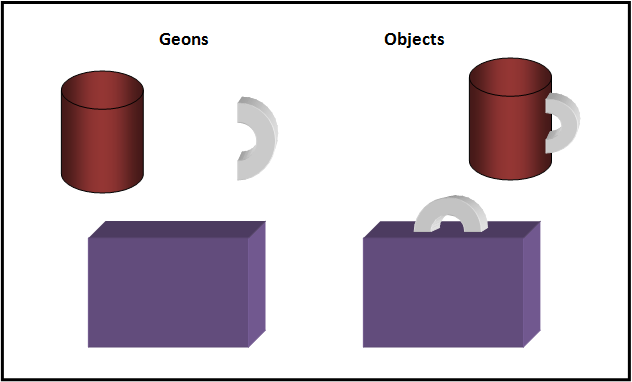
\includegraphics[width=\columnwidth]{res/fig/ANNgeonsObjects.png}
\caption{A set of geons and some of the objects that can be composed by them \cite{b10}.}
\label{fig8}
\end{figure}

In order to find evidences for this theory, Biederman tested human recognition system, mainly by using response time as empirical evidence. Hist tests shown that that varied visibility of geons and their connections clearly influence the way that the brain process the visual information. Main conclusions drawn in Biederman's research are \cite{b10}:

\begin{itemize}
\item Recognition is based on decomposition of an object in geons;

\item Recognition is more likely to be based on shape information than on color and texture;

\item  Recognition utilizes the relation among entities, in the form of orientation, distance, size and connections;

\item Intersections of lines making up geons are important for recognition, more so than having long untouched lines fully intact.

\end{itemize}

\subsection{Preprocessing}
The goal of the preprocessing step is to extract the shapes present in the image, which is performed in three steps. First we use an edge detection algorithm to find the edge pixels in the image. A second step uses the generated edge pixels to create the contours of the shapes and  in final step the resulting image of the second step will be used to extract the shapes that have now become visible.

The main motivation for the recognition by shapes is that in recognition of an object as a whole every discrepancy, even if it is only a small one, can disrupt the recognition process. As such, trying to recognize an object as a whole is possible as long as the object is not partly covered, or seen from a point of view that exposes a different side of the object than the system has been trained for. To make sure recognition can also take place in less perfect situations  the shapes can be rotated to a generalized position so that the number of possible projections of the shape onto the network is reduced to a subset of the possibilities present when a shape can appear in all of the different positions. 

To further reduce the number of positions the shape can be in, we can also attempt to remedy the mirroring possibility.
Often just small parts can indicate the presence of an object. For example, just the presence of a hand can indicate that there’s a person present or a set of wheels can give reason to believe a car might be in the scene. 
\\

\subsection{Representation}
After the preprocessing step, it will be created the representations of the shapes  for feeding them into a neural network. These representations can be  interpreted as shape descriptors or, just descriptors. A shape descriptor is a set of numeric values that describes the shape in a way that makes it distinguishable from other shapes. It is less sensitive to scaling or rotation of the shapes, so that a shape that is upside down can result in the same representation as a shape in normal position.
\\

\subsection{Interpretation}
Having a set of descriptor vectors of which each is about a hundred values long is a difficult basis for object recognition. This is why  the interpretation network should facilitate a reduction in this dimension, by somehow lowering the number of values to a short indication or description of the shape. The network will therefore take the descriptor of a shape as an input and output the classification of the shape. 
\\

\subsection{Learning process}
In order to train a neural network it would be a possibility to highlight every local shape of an object that is equal to a shape from another identical one, this  would lead to a great number of possible shapes, while the scope is to reduce this number as far as possible. 

\subsubsection{Associative mapping}
Associative mapping in which the network learns to produce a particular pattern on the set of input units whenever another particular pattern is applied on the set of input units. This can  be broken down into another two mechanisms:

\paragraph{auto-association}
an input pattern is associated with itself and the states of input and output units coincide. This is used to provide pattern completion, to produce a pattern whenever a portion of it or a distorted pattern is presented. In the second case, the network stores pairs of patterns building an association between two sets of patterns.

\paragraph{hetero-association}
is related to two recall mechanisms:

\begin{itemize}
\item nearest-neighbor recall, where the output pattern produced corresponds to the input pattern stored, which is closest to the pattern presented.

\item interpolating recall, where the output pattern is a similarity dependent interpolation of the patterns stored corresponding to the pattern presented. Yet another paradigm, which is a variant associative mapping is classification, when there is a fixed set of categories into which the input patterns are to be classified.
\end{itemize}

\subsubsection{Regularity detection}
Regularity detection in which units learn to respond to particular properties of the input patterns. Whereas in associative mapping the network stores the relationships among patterns, in regularity detection the response of each unit has a particular 'meaning'. This type of learning mechanism is essential for feature discovery and knowledge representation.

Modifying the knowledge stored in the network as a function of experience implies a learning rule for changing the values of the weights.
Information is stored in the weight matrix W of a neural network. Learning is the determination of the weights. Following the way learning is performed, we can distinguish two major categories of neural networks:

\begin{itemize}
\item fixed networks in which the weights cannot be changed, ie $\frac{\partial W}{\partial t} = 0$. In such networks, the weights are fixed apriori according to the problem to solve.

\item adaptive networks which are able to change their weights, ie  $\frac{\partial W}{\partial t} \neq 0$.
\end{itemize}

A first option is to use evolutionary techniques to find the best network. This option would be slightly preferred over random initialization, because it would work with several random networks and will enable us to retrieve the best of all their properties. A second option is to set the weights of the network randomly and leave them fixed. Although this process can lead to very different results, as soon as a network performs well it can be stored and used in all future cases. Another option was to come up with a set of primitive properties that are inherent to all shapes, classify a large set of many different shapes to these properties, and train the network to learn to indicate the presence or absence of these properties.

The objective is to create a system that is as autonomous and adaptable as possible. This excludes the actual labeling and classification of shapes that make up an object in advance. Furthermore, the adaptability of the system would be compromised by this process, since learning new shapes would also require these extra steps of categorizing shapes. 
Once a neural network is trained to a satisfactory level it may be used as an analytical tool on other data. To do this, the user no longer specifies any training runs and instead allows the network to work in forward propagation mode only. 

It is also possible to over-train a neural network, which means that the network has been trained exactly to respond to only one type of input; which is much like rote memorization. If this had happened, the learning process can no longer occur.

\subsection{Limitations}
Apart from defining the general architecture of a network and perhaps initially seeding it with a random numbers, the user has no other role than to feed it input and watch it train and await the output. 

It is also possible to over-train a neural network, which means that the network has been trained exactly to respond to only one type of input; which is much like rote memorization. If this had happened, the learning process can no longer occur.

\section{Conclusions}
This paper intention was to make a brief presentation of popular image recognition methods and algorithms used in this process.

Images can be analyzed in two ways. First method implies extracting global features from image content representation and the second and the more precise one implies local feature extraction. Global features aim to describe an image using all the pixels values for example color or texture, while local features aim to detect the interest points of the image and describe them in such a manner that they can be matched in other representations of the same scene.

In order to recognize an object we need to compute its interest points and descriptors which will be compare with a collection of images. We can train an artificial neural network to recognize the specific object based on specific patterns in its aspect. In order to make the network work we must feed it with a big set of representations of the same object in order to learn the objects aspects.

\begin{thebibliography}{00}

\bibitem{b1} Simon Achatz, Prof. Dr J¨org Conradt: ``State of the Art of Object Recognition Techniques''

\bibitem{b2} M. Hassaballah, Aly Amin Abdelmgeid and Hammam A. Alshazly: ``Image Features Detection, Description and Matching''

\bibitem{b3} Chris Harris , Mike Stephens: ``A COMBINED CORNER AND EDGE DETECTOR''

\bibitem{b4} Lowe, D.G. : ``Distinctive image features from scale-invariant keypoints'' Int. J. Comput. Vis. 60(2), 91–110 (2004)

\bibitem{b5}  Bay, H., Ess, A., Tuytelaars, T., Gool, L.: ``Speeded-up robust features (SURF)''. Comput. Vis. Image Underst. 110(3), 346–359 (2008)

\bibitem{b6} Gil Levi :``Binary descriptors'' www.gilscvblog.com 

\bibitem{b7} Alexandre Alahi, Raphael Ortiz, Pierre Vandergheynst: ``FREAK Fast Retina Keypoint''

\bibitem{b8} Michael Calonder, Vincent Lepetit, Christoph Strecha, and Pascal Fua: ``BRIEF: Binary Robust Independent Elementary Features''

\bibitem{b9} Ethan Rublee, Vincent Rabaud, Kurt Konolige, Gary Bradski: ``ORB: an efficient alternative to SIFT or SURF''

\bibitem{b10} Jelmer de Vries: ``Object Recognition:A Shape-Based Approach using Artificial Neural Networks''

\end{thebibliography}
\end{document}
